\documentclass[11pt,letterpaper]{article}
\usepackage[latin1]{inputenc}
\usepackage{amsmath}
\usepackage{amsfonts}
\usepackage{amssymb}
\usepackage{graphicx}
\usepackage{capt-of}

\setlength{\parskip}{1pc}
\setlength{\parindent}{0pt}
\setlength{\topmargin}{-3pc}
\setlength{\textheight}{9.0in}
\setlength{\oddsidemargin}{0pc}
\setlength{\evensidemargin}{0pc}
\setlength{\textwidth}{6.5in}

\title{6.170 Assignment 3 Documentation}
\author{Dina Betser}


\begin{document}
\maketitle

\section{Models}
\subsection{Object Models}
The object model for the problem domain is included in the figure below. The problem domain object model demonstrates the system that must be built. 

Some multiplicities that are not represented in the model are the number of \texttt{Box}es in a board, which is equal to $boardDim^2$, and the number of \texttt{HumanPlayer}s in the \texttt{VersusHumanMode}, which is 2.
\begin{center}
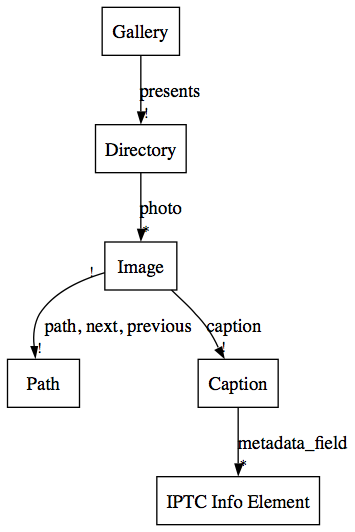
\includegraphics[width=9.5in, angle=90]{dot/obmod.png}
\label{fig:ob1} 
\end{center}

\subsection{State Machines}
The following state machine describes how the state of the application changes as game play progresses.
\begin{center}
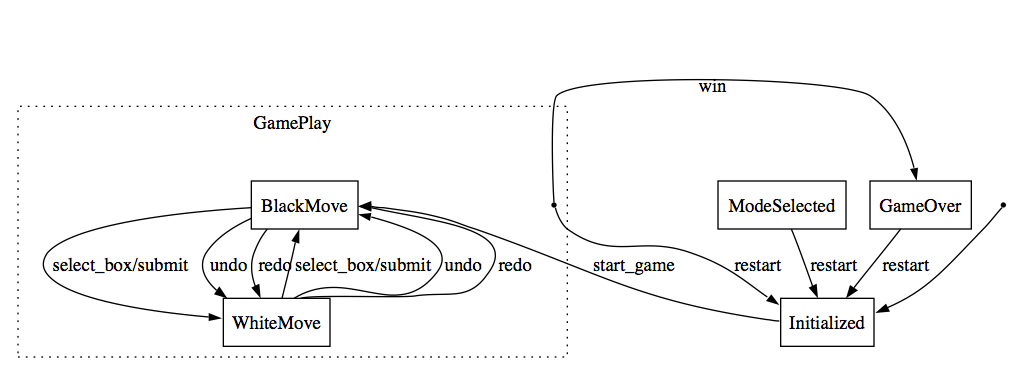
\includegraphics[width=7in]{dot/statediag.png}
\label{fig:sm1} 
\end{center}

\section{Design Notes}
\subsection{Key Challenges}
\begin{itemize}
\item One of the main challenges of this assignment was implementing the gameplay logic. Using online resources, I was able to get an idea of how the markers are reversed in according with the game rules.
\item Organizing the code to ensure that changes to the UI were not made directly from the \texttt{Game} ADT, which served as the main bulk of the model in the MVC format. Callbacks were crucial in achieving this result. Doing so supported Separation of concerns, and helped implement a View and Model that remained linked by a Controller entity.
\item Implementing undo/redo. This was done using a stack that stored \texttt{GameStateData} objects, each of which encapsulates the state of the board and the statistics of the game such as the current player and the number of boxes belonging to black, white, and still unallocated. 
\end{itemize}

\subsection{Issues Arising}
\begin{itemize}
\item How to implement undo and redo.\\
This required adding a way for a user to ``commit a transaction'', which was done using the ``Submit'' button. The Submit button ensured that the user was done with the current play before attempting to commit a move to change the state of the model. Upon submit, the state of the board was also recorded to the BoardStateHistory array. That array served as a stack to navigate during undo/redo. A pointer into the stack was kept such that the pointer always pointed to the last move committed, which could be decremented to get to previous states upon undo, and which would be incremented upon redo. In that way, the entire state of the board can be kept with every game.
\item How to switch players with human vs. human play.\\
Because I based my code structure on tictactoe.js, I 
\item A random player is selected to go first.\\
One issue the a
\item UI representation of markers.\\
In order to represent a marker state,
\end{itemize}

\subsection{Critique}
This project required a clear understanding of each Python class that was used. Each class I created had a clear specification and purpose, so the code itself was organized fairly well.

The \texttt{GameStateData} data structure was particularly succinct at storing all of the information required to store and restore the state of a game during undo/redo.

The implementation chose more sophisticated notions of undo/redo than required; for instance

The implementation also allowed a user to change play mode in the middle of the game, something that many implementations for this project did not.
\section{Specification}
\subsection{Overview}
This application generates a static HTML website that works as a browser-based photo gallery implementation. The gallery allows users to view photos stored locally to the directory where the script is run. Users may specify which metadata fields they wish to use as captions in the gallery. They may scan through the collection of images by clicking the left and right arrow buttons. All effects are achieved without the use of Jacascript; only HTML and CSS along with the Python Jinja2 library are used for this project.
\subsection{Key Features}
The key features of this implementation of the 6.170 photo gallery are:
\begin{itemize}
\item Minimalist, intuitive interface for scanning through photos in the gallery.
\item Images are displayed in the center of the UI, attracting attention. The caption is displayed below the photo, where users would expect it.
\item Generated HTML depends on multiple command-line arguments that can customize the files used and the output of the script.
\end{itemize}
\subsection{User Manual}
To run the code, python2.6 must be installed, with the jinja2 module and the iptcinfo module available.

The 6.170 photo gallery is a static HTML page that is generated via a Python script that uses the Jinja templating system. The HTML is generated by running a python script with command-line arguments specifying options.
For example, a sample run of the script to generate the html file photo\_gallery.html might look like:
\begin{verbatim}
$ python2.6 photo_gallery.py images/ photo_gallery.html caption/abstract
templates/photo_gallery_template.html
\end{verbatim}
In this case, the arguments are as follows:
\begin{verbatim}
$ python2.6 photo_gallery.py <image_directory> <output_filename> <comma-separated list of
metadata fields> <input_filename>
\end{verbatim}

The user may only specify a single directory from which to generate the gallery, and no subdirectories are included in the gallery. This image directory must be specified with a slash (\/) following the name.


\section{Implementation}

\subsection{Module Dependency Diagram}
This code's modules can only be seen as the member variables of classes, since there was only one Python module involved in the code generation.
\begin{center}
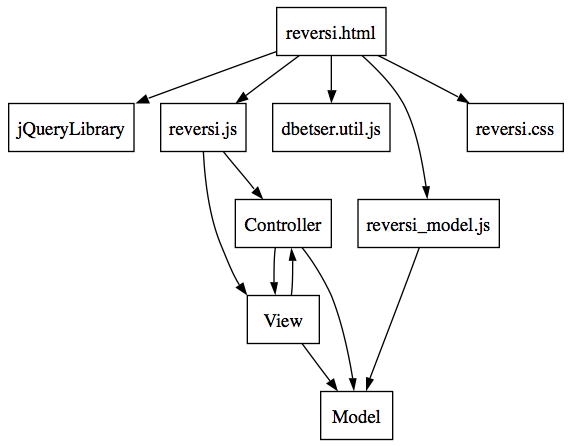
\includegraphics[width=250pt]{dot/moddepdiagram.png}
\label{fig:ob2} 
\end{center}
\subsection{Code Notes}
This code was fairly straightforward to write. The biggest issue I had was determining how to display only one photo, with previous and next buttons, using only HTML and CSS.

The most major hack that was included in the project deals with updating the player whose turn it is during undo/redo moves. One of the problems with my implementation was that 

\section{Testing}

\subsection{Test Plan}
To test the application, the generated HTML was inspected in multiple browsers, including Safari, Chrome, and Firefox.

The testing for this project was mostly manual since it was a more contained project.
\subsection{Test Cases}
To test the board itself, I did the following:
\begin{itemize}
\item hi
\end{itemize}

The captions are displayed even when multiple IPTCInfo elements are included. This was tested by including the caption/abstract element twice, which worked properly by including the photo abstract twice in the caption on the website.

The HTML was validated to ensure standards compliance.

All of the above was done in both the Firefox and Chrome browsers.

\subsection{Rationale and Conclusions}
This project fulfills the requirements of the assignment. The application runs as desired, and even implements undo/redo in a sophisticated and extensible way. Because I used extra slack days, I was able to debug to create a much cleaner and smoother product that I would have otherwise!

\end{document}

